When analyzing diffraction dat, not all of the pixels in 
an image should be used in the analysis. In order to make 
the program
ignore certain pixels when doing the analysis, this
program allows for two types of pixel masking:
threshold masking and polygon masking. You can 
apply either of these from the 
\gui{Masking} tab. figure~\ref{masking_tab}
shows this tab. 

\section{Threshold Masking}

\begin{SCfigure}[1][htbp]
    \centering
    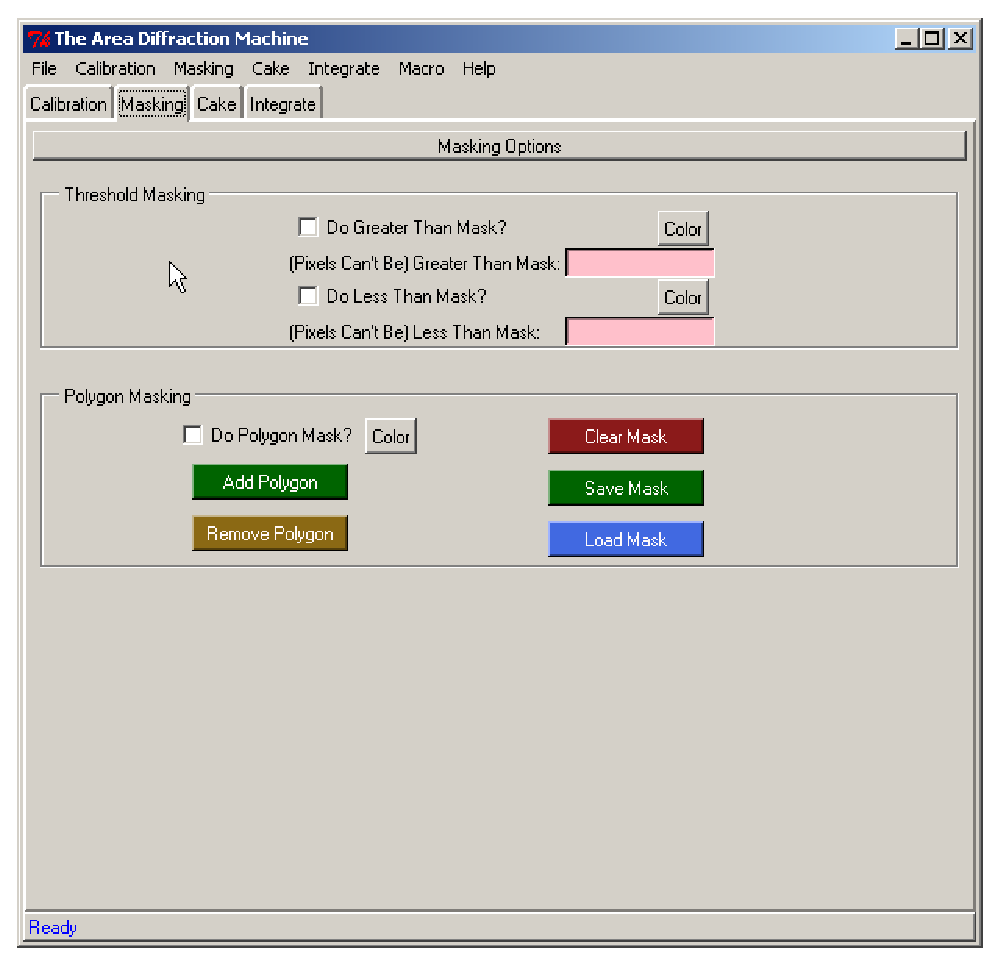
\includegraphics[scale=.75]{figures/masking_tab.eps}
    \caption{The pixel masking tab. It allows for threshold 
    masking and polygon masking.} 
    \label{masking_tab}
\end{SCfigure}

The top half of the \gui{Masking} tab is devoted to 
threshold masking. Threshold masking allows all pixels, 
either above a certain intensity or below a certain 
intensity, to be ignored when doing the diffraction 
analysis. The \gui{Do Greater Than Mask?} check box can 
be used to apply a mask that will cause all pixels 
greater than a certain value to be ignored.
The \gui{(Pixel's Can't Be) Greater Than Mask} input 
can be used to specify the maximum pixel value.
Correspondingly, the \gui{Do Less Than Mask} check box
can be used to make the program ignores all
pixels below a certain value. The particular value can 
be specified with the \gui{Less Than Mask} input. 

\begin{SCfigure}[1][htbp]
    \centering
    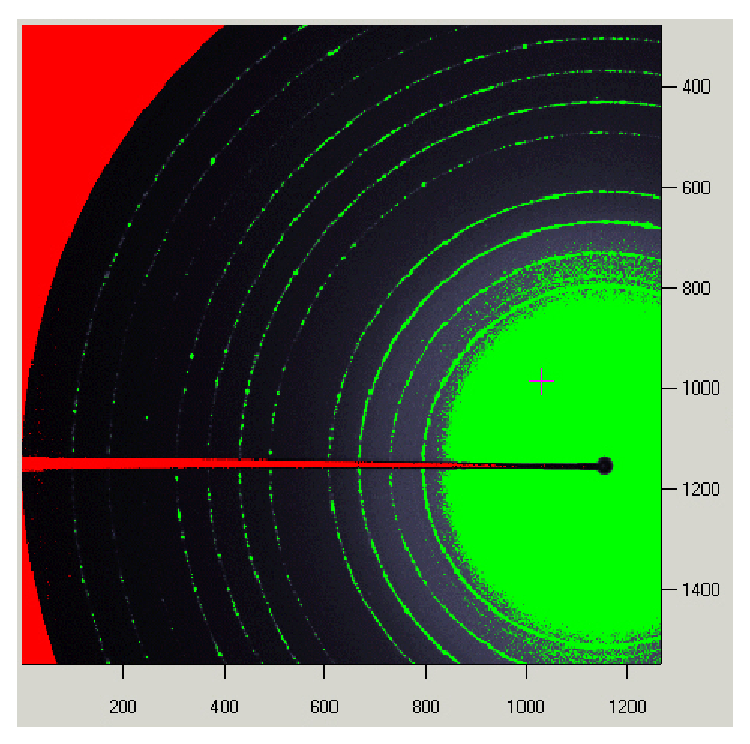
\includegraphics[scale=.75]{figures/Threshold_Masking.eps}
    \caption{A diffraction image with a
    greater than mask and less than mask.
    All pixels with intensity greater than 5000 
    have been colored green. All pixels with 
    intensity less than 30 have been colored red. Applying
    an intensity mask can be a useful way to see if a detector's
    pixels have been overloaded. They can also be a used to
    ensure that no overloaded pixels are used in subsequent
    data analysis.}
    \label{Threshold_Masking}
\end{SCfigure}

When you apply a threshold mask, the pixels over this threshold 
will all be colored differently on the diffraction and cake image. 
You can specify what you want these masked to be colored 
with the \gui{Color} button next to the greater 
than and less then masks. Figure~\ref{Threshold_Masking} shows 
what a diffraction image looks like when all pixels
with intensity above 5000 are colored green and all pixels 
below 30 are colored red.

When caked data is saved out to a file, any of the pixels 
that are larger than the greater than mask are saved 
as -2. Any of the pixels smaller than the less than mask
are saved as -3.  If you need to analyze caked data outside 
the program, this behaviour needs to be accounted for.

When an intensity integration is saved to a file, 
any of the too high or too low pixels are simply ignored when 
calculating average intensity. 

\section{Polygon Masking}

\begin{SCfigure}[1][htbp]
    \centering
    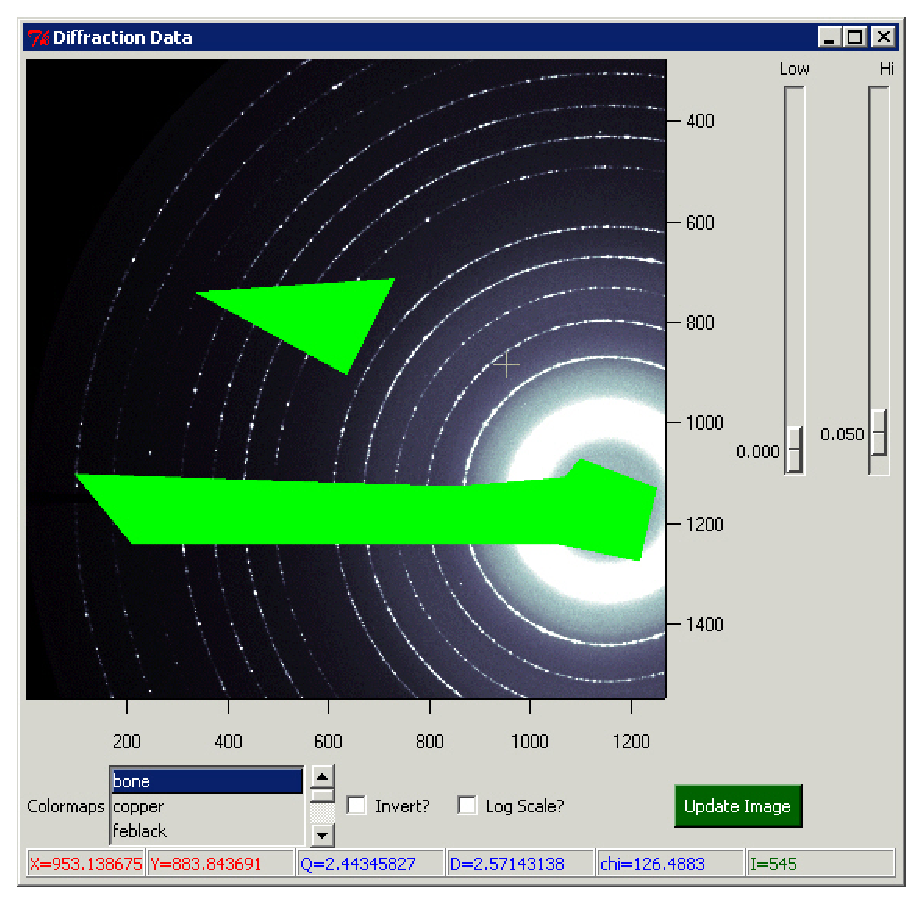
\includegraphics[scale=.75]{figures/Displayed_Polygon.eps}
    \caption{Here are two polygon masks that have been applied
    to a diffraction image. One of them blocks the beam stop.}
    \label{Displayed_Polygon}
\end{SCfigure}

Sometimes, large areas of a diffraction image should not
be included in any data analysis. For example, 
often a beam stop blocks part of the detector
and the pixels behind the beam stop should be ignored. 
To allow for this sort of masking, the program has a 
polygon masking feature. Polygons can be drawn around 
certain parts of the diffraction image and those parts 
of the image will not be used in any subsequent analysis. 
This program can handle multiple polygons at the same time.

So long as the \gui{Do Polygon Mask?} check box is
selected, the polygon masks will be used 
when performing subsequent analysis. 
The polygons will be displayed on the diffraction and cake image. 
Any pixel in the diffraction or cake image that is inside one of
the polygons will have a different color.
An example of polygons on a diffraction image are 
shown in figure~\ref{Displayed_Polygon}.
The color of the polygon masks can be changed using 
using the \gui{Color} button
next to the \gui{Do Polygon Mask?} check box.
When caked data is saved out, any pixels inside 
polygon masks will be given an intensity 
value of -4. During an intensity integration 
masked pixels will be ignored.

\begin{SCfigure}[1][htbp]
    \centering
    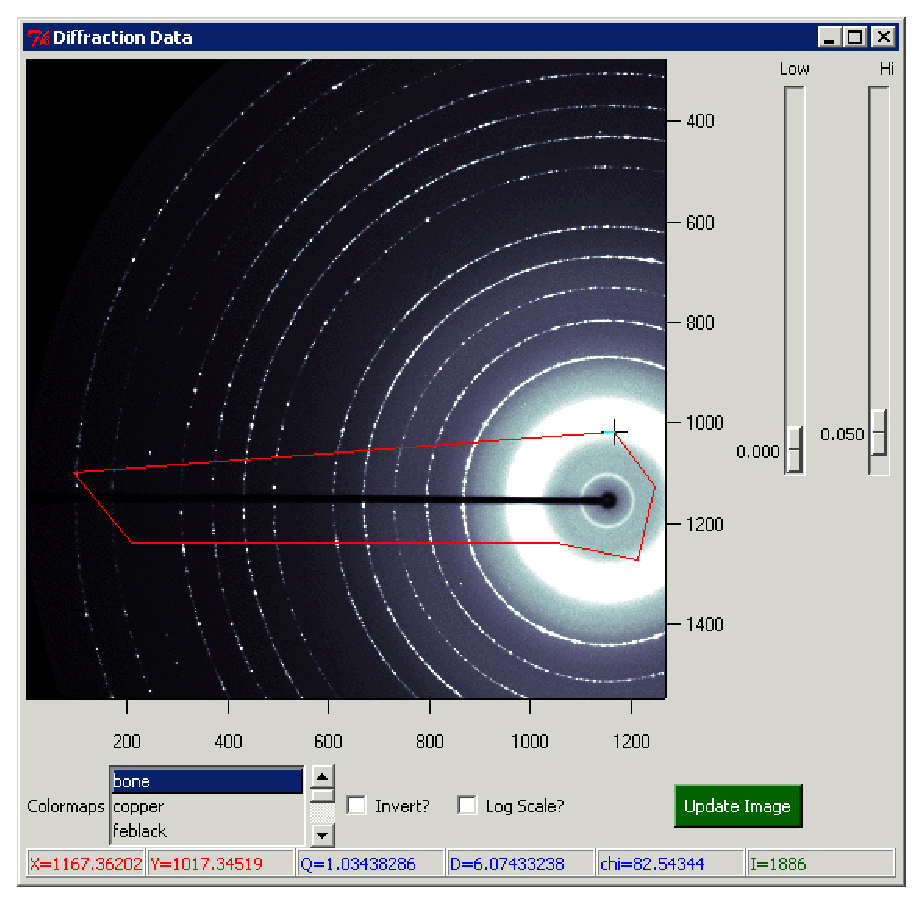
\includegraphics[scale=.75]{figures/Adding_Polygon.eps}
    \caption{Here is the interface for adding a new polygon 
    mask to the program. This particular mask will cover 
    the beam stop so that the beam stop does not affect
    the intensity integration.}
    \label{Adding_Polygon}
\end{SCfigure}

A polygon mask can be added to the image by pushing
the \gui{Add Polygon} button on the \gui{Masking} tab. 
This button will stay down when pushed.  Pushing it puts 
the program in polygon drawing mode.  In this mode, the 
diffraction image will behave differently. The diffraction
image can no longer be zoomed or panned.
Instead, left clicking on the diffraction image will make
the program draw the polygon.  The first left click adds the
first vertex. Each success left click add another vertex. 
The drawing can be finished by right clicking (this will
also create a final vertex). Right clicking will make
the program exit the drawing mode, return to its
original state, and add the polygon into the program. 
Multiple polygons can be added using the \gui{Add Polygon}
button. Figure~\ref{Adding_Polygon} shows 
the program when a polygon is
being drawn. Drawing a polygon can be aborted without
saving the mask by unpushing the \gui{Add Polygon} button.

\begin{SCfigure}[1][htbp]
    \centering
    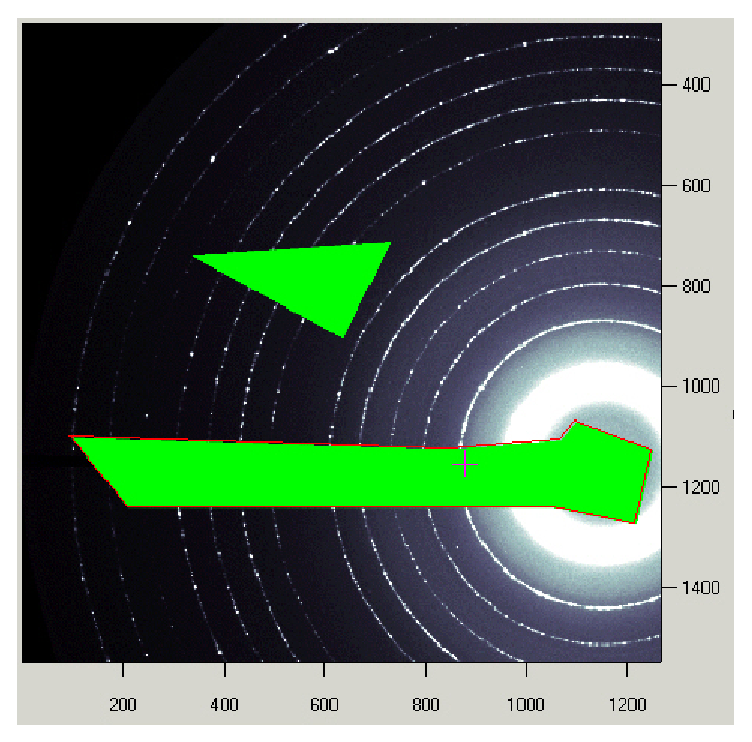
\includegraphics[scale=.75]{figures/Removing_Polygon.eps}
    \caption{Here is the diffraction
    image window as a polygon is about to be removed.
    When mousing over a polygon to remove it,
    the program will display a red border around it.}
    \label{Removing_Polygon}
\end{SCfigure}

The \gui{Remove Polygon} button can be used to remove
a polygon in the program. Like the \gui{Add Polygon} 
button, this button will stay pushed and change the
behavior of the diffraction image. After the 
\gui{Remove Polygon} button is pushed, clicking over
a particular polygon will remove it.
After the polygon is removed, the program will 
return to its normal state.
Figure~\ref{Removing_Polygon} shows what the diffraction
window looks like when a polygon is about to be removed.
The program can be returned to its normal state without
removing a polygon by unpushing the \gui{Remove Polgyon}
button.

The \gui{Clear Mask} button can be used to remove
all the polygons at once. The \gui{Save Mask} button
can be used to save all the polygons to a file.
A file of polygons can be added to the program 
using the 
\gui{Load Mask} button. The file for polygon
files is very simple. For the polygons in 
figure~\ref{Displayed_Polygon}, the following
file would be saved:
\begin{lstlisting}[caption={'polygons.dat'}]
# Polygon(s) drawn on Thu Feb 07 00:00:21 2008
93.140587183	1098.06704199
208.013978042	1237.77792276
1052.48863517	1237.77792276
1213.93231962	1271.92947139
1248.08386825	1126.00921814
1095.95424252	1067.02017959
1064.90738013	1104.27641447
847.579343365	1122.9045319

332.201427619	737.923438212
633.355992844	902.471808902
729.601266267	709.981262058
\end{lstlisting}
Each line is an ($x$,$y$) coordinate for one of 
the nodes of a polygon.  The coordinates are separated
by spaces. Each polygon is separated by a newline.  
Comment lines beginning with \# are 
ignored. 

\section{Masking Caked Plots}

\begin{figure}[htb]
    \centering
    \subfloat[A rectangular polygon mask in 
    the middle of a diffraction image]{
    \label{box_mask_diffraction}
    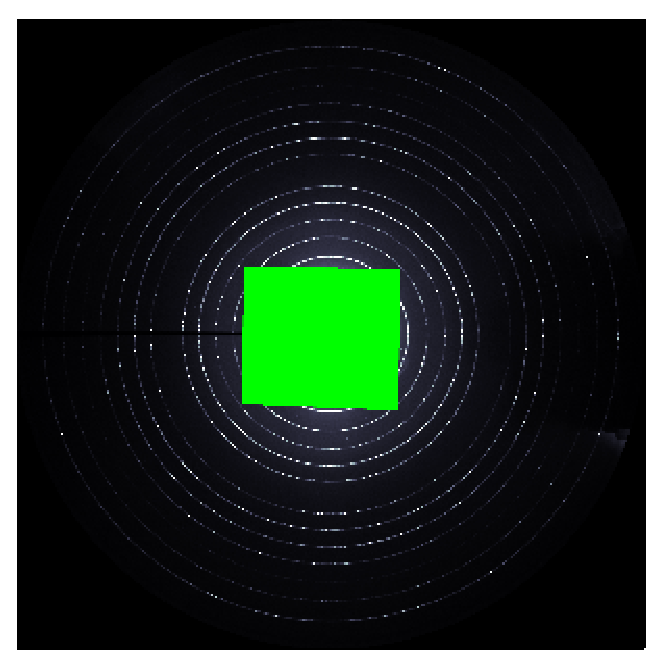
\includegraphics[scale=.75]{figures/box_mask_diffraction_image.eps}}\;\;
    \subfloat[The same rectangular mask on
    a caked plot]{
    \label{box_mask_cake}
    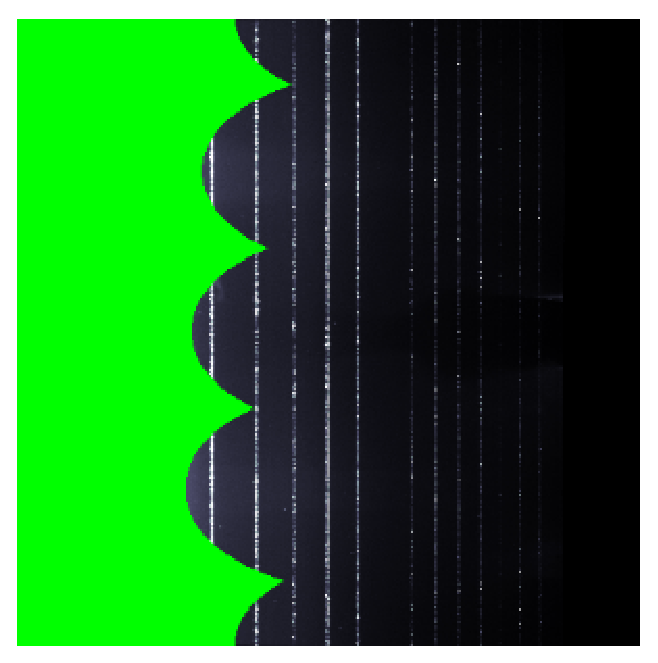
\includegraphics[scale=.75]{figures/box_mask_cake_image.eps}}
    \caption{An example of how a relatively simple
    shape on a diffraction image will can look very
    different on a caked plot.}
    \label{box_mask}
\end{figure}

Any polygon mask or threshold mask will also 
show up on the caked plot. Polygons on the 
diffraction image can look very distorted on 
caked plots. Figure~\ref{box_mask} shows an example.



